\section{Exercise 4}

\subsection{Analytical value of $\text{Var}(X(t))$}

For a Wiener process $W(t)$, consider the process:
\begin{equation*}
X(t) = W(t) - \frac{t}{T}W(T-t), \quad \text{for } 0 \leq t \leq T.
\end{equation*}

For the definition of the Wiener process, it is known that $\mathbb{E}[W(t)]=0$ and $\text{Var}(W(t))=t$. \\

Firstly, the expectation of $X(t)$ is computed
\begin{align*}
\mathbb{E}[X(t)] &= \mathbb{E}\left[W(t) - \frac{t}{T}W(T-t)\right] \\
&= \mathbb{E}[W(t)] - \frac{t}{T}\mathbb{E}[W(T-t)] \\
&= 0 - \frac{t}{T} \cdot 0 = 0
\end{align*}

Next, the variance of $X(t)$ is derived as follows
\begin{equation*}
\text{Var}(X(t)) = \mathbb{E}[X^2(t)] - (\mathbb{E}[X(t)])^2 = \mathbb{E}[X^2(t)]
\end{equation*}

Expanding $X^2(t)$, I find that
\begin{align*}
X^2(t) &= \left(W(t) - \frac{t}{T}W(T-t)\right)^2 \\
&= W^2(t) - 2\frac{t}{T}W(t)W(T-t) + \frac{t^2}{T^2}W^2(T-t)
\end{align*}

Taking the expectation,
\begin{align}
\mathbb{E}[X^2(t)] &= \mathbb{E}[W^2(t)] - 2\frac{t}{T}\mathbb{E}[W(t)W(T-t)] +
                      \frac{t^2}{T^2}\mathbb{E}[W^2(T-t)] \label{eq:expX2}
\end{align}

Using the properties of the Wiener process stated before, I can simply find that
\begin{align}
\mathbb{E}[W^2(t)] = t \qquad \text{and} \qquad \mathbb{E}[W^2(T-t)] = T-t \label{eq:expvarW}
\end{align}

To compute $\mathbb{E}[W(t)W(T-t)]$, the property of independent increments of the Wiener process is used. \\

Assume $s \leq t$. Then, it is possible to decompose $W(t)$ as $W(t) = W(s) + (W(t) - W(s))$.
Since $W(t) - W(s)$ is independent of $W(s)$ and has mean zero,
\begin{align*}
\mathbb{E}[W(s)W(t)] &= \mathbb{E}[W(s)(W(s) + (W(t) - W(s)))] \\
&= \mathbb{E}[W(s)^2] + \mathbb{E}[W(s)(W(t) - W(s))] \\
&= s + 0 = s
\end{align*}

Thus, for $s \leq t$, we have $\mathbb{E}[W(s)W(t)] = s$. By symmetry, for $t \leq s$, we have $\mathbb{E}[W(s)W(t)] = t$. Therefore, in general $\mathbb{E}[W(s)W(t)] = \min(s, t).$
Applying this result to $\mathbb{E}[W(t)W(T-t)]$, substituting $s = t$ and $t = T - t$, it follows that
\begin{equation*}
    \mathbb{E}[W(t)W(T-t)] = \min(t, T - t)
\end{equation*}

This gives the piecewise expression:
\begin{align}
\mathbb{E}[W(t)W(T-t)] = 
\begin{cases}
t, & \text{if } t \leq \frac{T}{2}, \\
T - t, & \text{if } t > \frac{T}{2}. \label{eq:covW}
\end{cases}
\end{align}

Now that all the values are finally known, it is possible to substitute the results (\ref{eq:expvarW}) and (\ref{eq:covW}) into the expression (\ref{eq:expX2}), obtaining
\begin{align*}
\mathbb{E}[X^2(t)] &= t - 2\frac{t}{T}\min(t, T-t) + \frac{t^2}{T^2}(T-t).
\end{align*}

Thus, the variance of $X(t)$ is given by the expression
\begin{equation*}
\text{Var}(X(t)) = t - 2\frac{t}{T}\min(t, T-t) + \frac{t^2}{T^2}(T-t).
\end{equation*}

In particular for $T = 10$, this simplifies to
\begin{equation}
\text{Var}(X(t)) = 
\begin{cases}
t - \frac{t^2}{5} + \frac{t^2(10-t)}{100}, & \text{if } t \leq 5, \\
t - \frac{t(10-t)}{5} + \frac{t^2(10-t)}{100}, & \text{if } t > 5. \label{eq:var_t}
\end{cases}
\end{equation}

\subsection{Numerical Simulation}

 For numerical confirmation, I simulated 100000 paths of $X(t)$ and estimated the variance in 1000 time steps over the time interval $[0,T]$ with $T = 10$. The Wiener process $W(t)$ was approximated by generating random increments, which were then accumulated to produce a discretized representation of the continuous process. This discretized process was used to compute the values of $X(t)$ at each time step.

To estimate the variance of $X(t)$, the sample variance was calculated across all simulated paths at each time step. Then, this numerical estimate was compared with the analytical expression (\ref{eq:var_t}) derived before.

\begin{figure}[h!]
\centering
\begin{minipage}{0.5\textwidth}
    \centering
    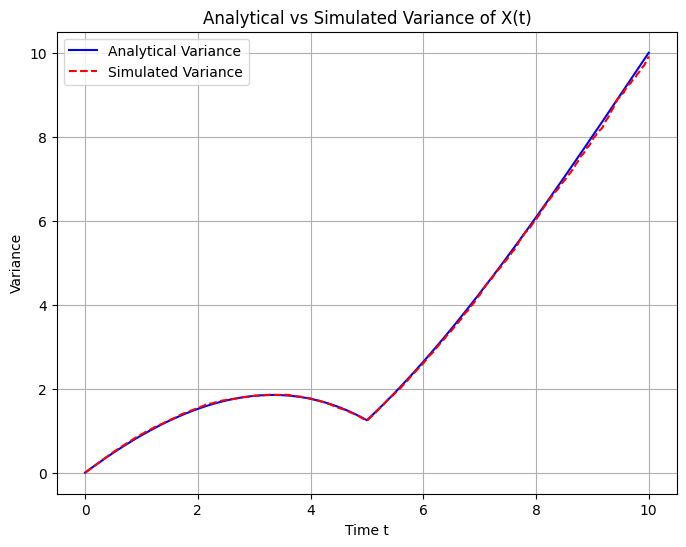
\includegraphics[width=1\textwidth]{Exercise_set_01/img/AnalyticalVsSimulated.png}
    \caption{Analytical vs Simulated Variance of \(X(t)\)}
    \label{fig:var}
\end{minipage}%
\begin{minipage}{0.5\textwidth}
    \centering
    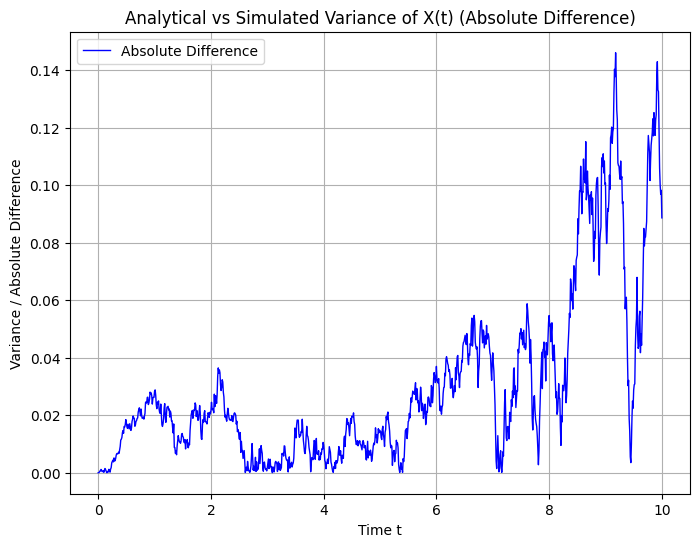
\includegraphics[width=1\textwidth]{Exercise_set_01/img/AnalyticalVsSimulated_abs.png}
    \caption{Absolute Difference Between Analytical and Simulated Variance of \(X(t)\)}
    \label{fig:diff}
\end{minipage}
\end{figure}

The results show agreement between the simulated and analytical variances, as shown in Figure \ref{fig:var}. However, in Figure \ref{fig:diff} it is possible to see accuracy differences between $t\leq5$ and $t\leq10$. In fact, for $t \leq 5$, the difference remains consistently low and stable, indicating a high level of precision in this region. Instead, for $t \geq 5$, the error begins to increase slightly, with a more noticeable rise as $t$ approaches $T=10$. In conclusion, it seems that the accuracy is sensitive to $t$.